%-------------- Oliver Pharr  ODR  -------

\section{Oliver Pharr with ODR}
For a definition of the Oliver Pharr method see \cite{OliverPharr}. \\ 
This method is shown unless the software was compiled without Fortran support.  \\

\begin{figure}[ht]
  \centering
  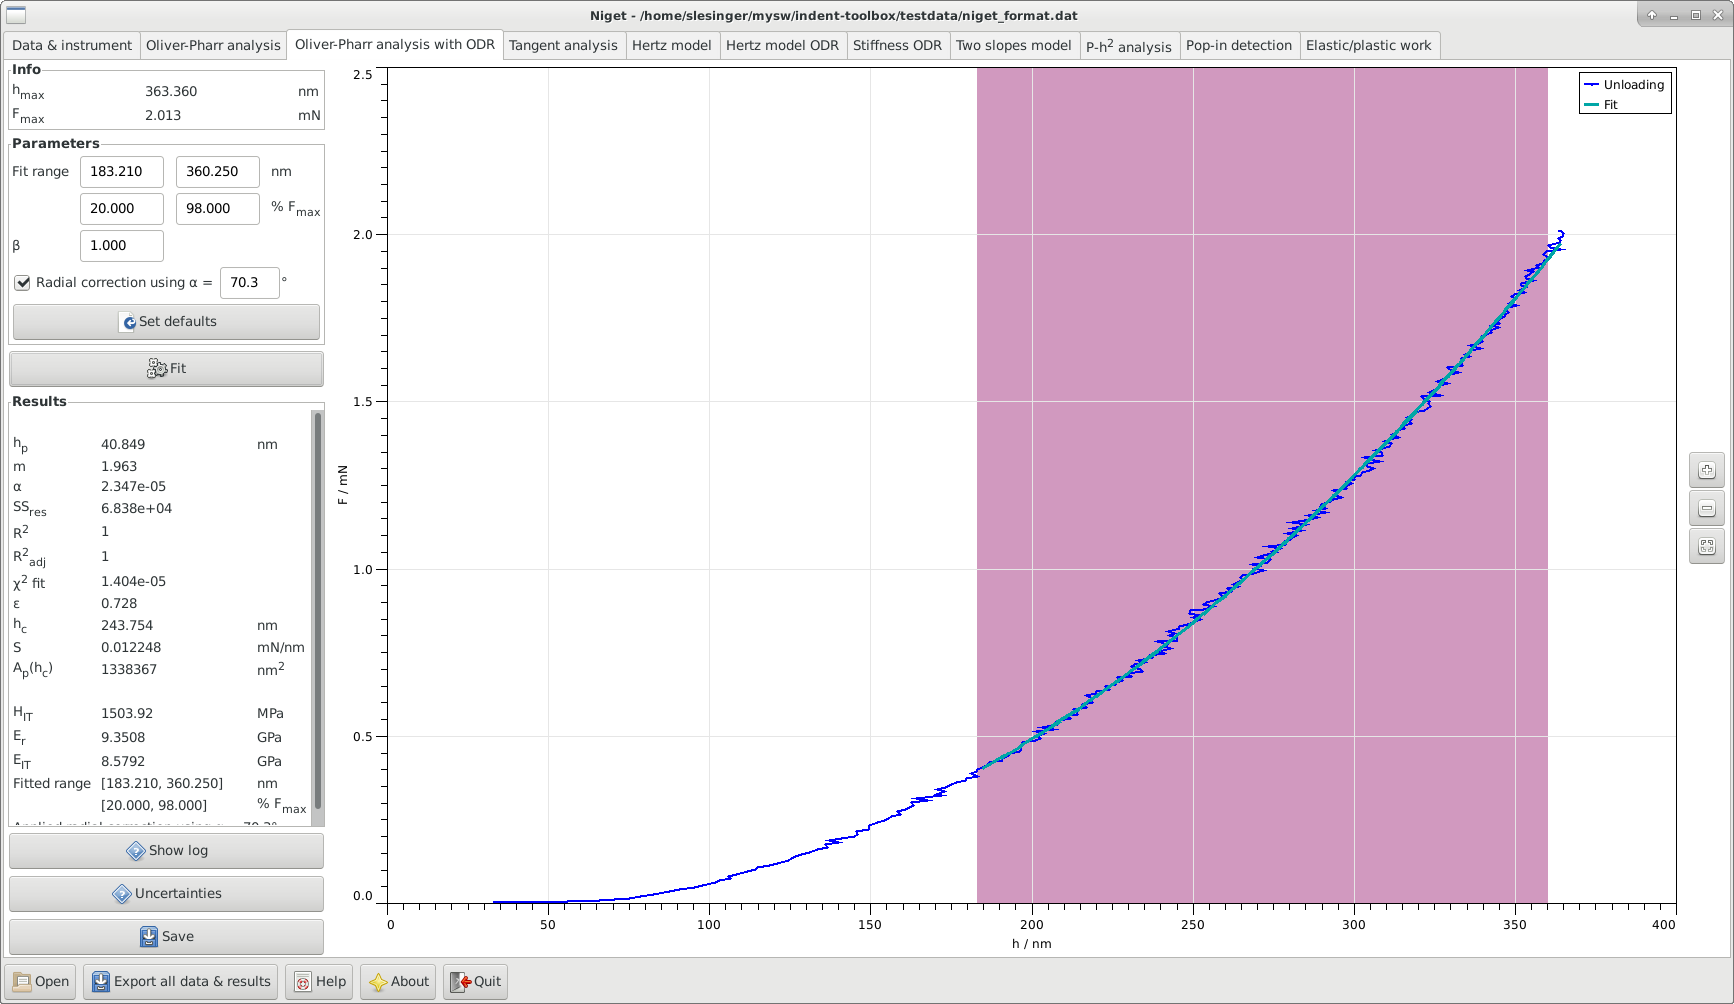
\includegraphics[width=\textwidth]{images/screen-op-odr}
  \caption{Oliver-Pharr analysis using orthogonal data regression}
\end{figure}

\subsection{Window}
The window consists of several blocks:
\begin{itemize}
 \item \emph{Info} displays the maximum depth and force during the indentation
 \item \emph{Parameters} shows the selected range in nm and in \% of the maximum force, the correction $\beta$, and the radial correction. 
        \begin{itemize}
          \item[-] The fitting range can be selected either using the mouse or typing in the range entries. The range can be defined either in nm or in percent of the maximum force. 
                   It is often recommended to use the range 40--98 \% F$_\mathrm{max}$ for the fit, see section \ref{opodr_calc}.  
          \item[-] The parameter $\beta$ accounts for any deviations from the axisymmetric case and is used in the calculation of the reduced modulus in equation \eqref{eq:Er}. 
                   Currently, the default value is no correction $\beta = 1.0$. The value supplied by the user is saved in the settings and can be reset to its default value.
                 \item[-] Optional radial correction of calculated hardness and modulus values according to ISO 14577-1:2015. The angle $\alpha$ denotes the cone-equivalent angle between the tip side and axis. For a Berkovich tip, $\alpha = 70.3^\circ$.
                   \item \emph{Set defaults} button resets the fitting range, the beta value, and radial correction settings according to recommendations provided in ISO 14577-1.
          \end{itemize}
 \item \emph{Fit} button, see section \ref{opodr_calc} for details of the calculation.
 \item \emph{Results} displays all results in the following order: the residual depth $\hp$, the power $m$ of the power law function, the parameter $\varepsilon$, 
       the contact depth  $\hc$, the slope $S$, the contact area $\Ap(\hc)$, the indentation hardness $H_{IT}$, the contact modulus $E_r$, the indentation modulus $E_{IT}$ and the ranges used for the fitting procedure.
       The variables are described in detail in section \ref{opodr_calc}. If the fittings procedure failed a warning is shown.
 \item \emph{Uncertainties} show the uncertainty analysis window, see section \ref{opodr_unc}.
 \item \emph{Show log} Show the report about the fitting procedure in a separate window.  The reports are saved to files \emph{fit.log.op.err} and \emph{fit.log.op.rpt}. 
 \item \emph{Save} save parameters and results to given file. 
 \item \emph{Graph} display the unloading curve and the fitted curves. Stepwise zooming/unzooming can be performed by selecting a range with the mouse and pressing the \emph{Zoom}/ \emph{Unzoom} buttons. The graph is restored to its original size by the \emph{Restore} button.
\end{itemize}

\subsection{Procedure} \label{opodr_calc}
This is a slight modification of the standard Oliver Pharr method described in section \ref{op_calc} using a better fitting procedure. 
\begin{enumerate} 
 \item 
 Fit the upper part of the unloading curve with a power law function
$$
F = \alpha (h - \hp)^m.
$$
using orthogonal least squares as implemented in the package ODRPACK95 \cite{odrpack95}. The range should be approx. 40--98 \% F$_\mathrm{max}$. All three parameters are fitted.
\item  Same as steps 3--4 in \ref{op_calc}.
\item If the radial correction is on, the hardness and reduced modulus are found by iterating the following relations
\begin{eqnarray}
 H^n &=& H^0 \left(1+K \frac{H^{n-1}}{E_{IT}^{n-1}}\right)^2 \\
 E_r^n &=& E_r^0 \left(1+K \frac{H^{n-1}}{E_{IT}^{n-1}}\right)
\end{eqnarray}
where $H^0$ and $E_r^0$ are the initial estimates obtained from step 4 in section \ref{op_calc}. The iteration limit is set to a relative difference $0.5 \cdot 10^{-4}$
Young's modulus is updated in each step according to \eqref{eq:Eit} and $K$ is the radial correction factor computed from Poisson's ratio and the angle between tip sides and axis $\alpha$
\begin{equation}
 K = \frac{1-2 \nu}{2(1+\nu)} \sin \alpha.
\end{equation}
The area function is corrected with the final values of hardness and modulus as 
\begin{equation}
 A = A^0 \left(1+K \frac{H}{E_{IT}}\right)^2.
\end{equation}




\end{enumerate}
